\subsection{Процессы инициации, планирования, реализации проекта}

\textit{Инициация проекта}, являясь одной из важнейших его фаз, закладывает фундамент успеха всего проекта.
Здесь определяются основные цели проекта, анализируются стратегические риски, выделяются ключевые участники проекта, определяются общие принципы организации управления проектом.

В состав процессов инициации входят:
\begin{itemize}
	\item  разработка устава проекта;
	\item  анализ заинтересованных сторон;
	\item  сбор требований;
	\item  стартовое совещание по проекту.
\end{itemize}

Основными задачами в ходе инициации проекта являются:
\begin{itemize}
	\item понимание основных заинтересованных сторон проекта, их интере­сов и ожиданий от проекта и его результатов;
	\item сбор требований от заказчика и иных заинтересованных сторон;
	\item формальный авторизованный старт проекта путем выпуска до­кумента <<Устав проекта>> и проведения стартового совещания по
	проекту.
\end{itemize}

Рассмотрим процессы инициации проекта более подробно.

Разработка устава проекта.
Целью разработки устава проекта является авторизация и формализа­ция проекта путем четкого очерчивания границ проекта, документиро­вания его целей и результатов, определения менеджера проекта, зоны его ответственности и полномочий.
Устав проекта должен связать проект со стратегическими целями организации, обосновать его необходимость, определить его содержа­ние и ответственных за реализацию.

Целью устава проекта, как исходного интеграционного документа является обеспечение однозначного понимания и фиксация:
\begin{itemize}
	\item  обоснование инициации проекта;
	\item  цели и результаты проекта;
	\item  описание и структуру продукта проекта;
	\item ожидания ключевых участников проекта;
	\item критерии успеха проекта;
	\item фамилию менеджера проекта и зону его ответственности в проекте;
	\item основные принципы организации проекта и управления им.
\end{itemize}

Устав проекта --- документ, разработка которого направлена на обеспечение следующих результатов:
\begin{itemize}
	\item авторизацию проекта;
\item определение проекта;
\item назначение менеджера проекта и распределения ролей основных участников проекта.
\end{itemize}

Результатами процесса разработки устава проекта являются однознач­ное понимание содержания проекта всеми его участниками и автори­зация начала проекта лицами, принимающими решение \cite[135--137]{polkovnikov}

Анализ заинтересованных сторон.
Целью анализа заинтересованных сторон является понимание возмож­ных зон воздействия на проект со стороны его участников и внешних заинтересованных сторон путем выявления основных лиц, групп и организаций, имеющих прямые или косвенные интересы в проекте.

Заинтересованные стороны (стейкхолдеры) в проекте существуют независимо от нашего желания.
Если бы их не было, проект никогда бы не состоялся.
При этом и х интересы весьма различаются.
Одни заинтересованные стороны проект запускают, продвигают к успеху, другие стороны имеют иные интересы.

Интересы по отношению к проекту могут быть:
\begin{itemize}
	\item положительными или отрицательными;
	\item прямыми или косвенными;
	\item явными и неявными (скрытыми).
\end{itemize}

Действия заинтересованных сторон иногда способствуют успеху проекта, а иногда --- нет.
Заинтересованные стороны будут влиять на окружение проекта (см. рисунок \ref{fig:okuzhenie}), создавая для менеджера проекта либо позитивные условия, либо серьезные препятствия для успеха проекта.

\begin{figure}[h]
	\centering
	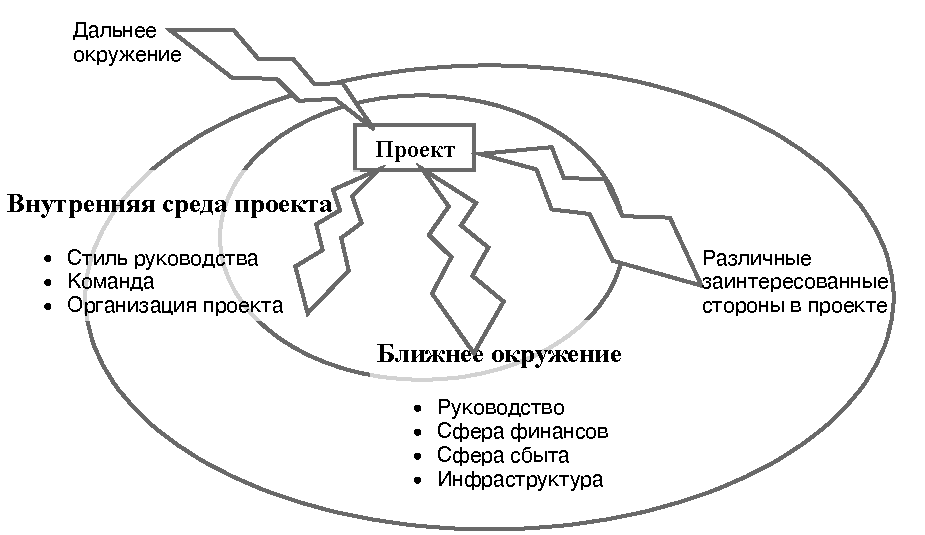
\includegraphics[width=\linewidth]{okruzh}
	\caption{Окружение проекта}
	\label{fig:okuzhenie}
\end{figure}

Выделяют ближнее и дальнее окружение проекта.
В ближнем окружении основными заинтересованными сторонами являются руко­водство организации, представители функциональных подразделений,
сотрудники, в дальнем --- конкуренты, органы власти, представители общественных организаций.

В ходе анализа заинтересованных сторон в проекте рекомендуется выделить основные группы заинтересованных сторон и понять их ин­тересы.
Это требуется:
\begin{itemize}
	\item для назначения явных заинтересованных сторон (участников про­екта) на роли, соответствующие их интересам;
	\item согласования с ключевыми внутренним и (а иногда и внешними) заинтересованными сторонами целей и результатов проекта;
	\item выявления угроз и зон риска со стороны заинтересованных сторон, негативно настроенных по отношению к проекту;
	\item определения потенциальных возможностей (в том числе дополни­тельных), возникающих в случае активного привлечения соответ­ствующих заинтересованных сторон;
	\item установления информационных потребностей заинтересованных сторон и дальнейшего включения их в коммуникационное поле проекта.
\end{itemize}

Результатами процесса анализа заинтересованных сторон являются готовность менеджера и команды проекта к влиянию, оказываемому на проект различными заинтересованными сторонами, и минимизация негативных эффектов этого влияния.

Заинтересованные стороны и их интересы могут быть отражены в Реестре заинтересованных сторон.
Для каждой заинтересованной стороны в этом документе полезно зафиксировать:
\begin{itemize}
	\item имя человека или название группы, представляющих заинтересо­ванную сторону;
	\item отношение заинтересованной стороны к проекту (положительное, отрицательное, нейтральное);
	\item силу возможного влияния на проект;
	\item степень информированности о проекте, его целях и текущем со­стоянии;
	\item дополнительные условия, при которых отношение к проекту может измениться.
\end{itemize}

По итогам анализа заинтересованных сторон проекта могут быть внесены изменения в существующие проектные документы: Устав,
План проекта и др. \cite[141--143]{polkovnikov}.

Сбор требований.
Целью процесса сбора требований является достижение более пол­ного, четкого и однозначного понимания целей и результатов проекта, а также ожиданий заказчика и иных заинтересованных сторон в ча­сти, касающейся функциональных, технических, пользовательских и иных характеристик продукта проекта.

Необходимо получить, понять, проанализировать и документаль­но зафиксировать требования основных заинтересованных сторон, которые могут повлиять на содержание проекта и организацию его выполнения.

Требования могут относиться к любым аспектам проекта:
\begin{itemize}
	\item целям и результатам;
	\item продукту проекта и его характеристикам;
	\item жизненному циклу проекта, этапам или составным элементам проекта;
	\item условиям реализации проекта и правилам выполнения отдельных работ;
	\item схемам финансирования или привлечения средств;
	\item условиям взаимодействия между участниками;
	\item правилам приемки продукта или сдачи результатов промежуточ­ных этапов и др.
\end{itemize}

Чаще всего требования распространяются на цели и результаты, а также на продукт проекта.
Основную роль в определении требова­ний играют ключевые заинтересованные стороны, в первую очередь заказчик.

Кроме того, при определении требований к продукту проекта важ­ным является понимание таких заинтересованных сторон, как поль­зователи, будущие покупатели (клиенты), эксплуатирующая орга­низация.

Результатом процесса сбора требований должна стать минимизация дополнительных требований и пожеланий заказчика по отношению к продукту проекта и проекту в целом, возникающих в ходе его реализа­ции.
В идеальной ситуации их не должно быть совсем. Как следствие, это должно привести к минимизации внесения изменений в проект на более поздних этапах.

Иногда по итогам процесса сбора требований создается документ Требования к продукту или Технические требования к проекту.
В зависимости от содержания проекта название документа может из­меняться \cite[143--144]{polkovnikov}.

Стартовое совещание по проекту.
Целью стартового совещания по проекту является информирование всех заинтересованных сторон проекта об основных решениях, приня­тых в ходе инициации проекта, и согласование с ними утверждаемых проектных документов.

Эффективно проведенное стартовое совещание может дать мощный импульс всему проекту и задать верное направление работе команды проекта.

В повестку дня стартового совещания по проекту рекомендуется включить следующие пункты:
\begin{itemize}
	\item представление менеджера проекта, куратора и заказчика;
\item знакомство участников;
\item идея и замысел проекта, предпосылки и обоснование его запуска;
\item основные положения Устава проекта;
\item распределение ролей в команде проекта и степени загрузки участ­ников в проекте;
\item принципы организации и взаимодействия в проекте.
\end{itemize}

Присутствие на стартовом совещании по проекту куратора, заказ­чика и иных важных участников поднимет статус проекта и статус менеджера проекта в глазах членов проектной команды.

Согласование с командой целей и результатов, принципов работы и взаимодействия позволит вовлечь участников в процесс управления и принятия решений по проекту, что должно повысить их ответствен­ность и мотивацию.

Результатом стартового совещания по проекту должно стать четкое, общее и одинаковое понимание участниками проекта его целей и за­дач, текущего статуса, системы организации проекта и своего места в команде начинающегося проекта \cite[145]{polkovnikov}.

Начало проекта закладывает фундамент всех его успехов.
Ошибки, допущенные в ходе инициации, обязательно напомнят о себе в даль­нейшем.
К числу самых распространенных ошибок, случающихся в начальной стадии проекта, относятся:
\begin{itemize}
	\item нечеткое понимание целей и границ проекта;
\item неформализованный подход к запуску проекта;
\item необоснованный запуск проекта.
\end{itemize}

\textit{Планирование проекта} --- процесс поиска и расчета оптимального способа достижения целей проекта.

В ходе планирования необходимо по воз­можности четко ответить на вопросы: кто, когда, как и какие работы должен выпол­нить для достижения целей проекта.

Ответы на эти вопросы ищутся и находятся в ходе последовательной разработки Плана проекта --- единого сводного документа, со­держащего результаты планирования основ­ных функциональных областей проекта:
\begin{itemize}
	\item сроков;
\item стоимости;
\item персонала;
\item поставок;
\item рисков;
\item коммуникаций и др.
\end{itemize}

Процессы планирования --- процессы, осуществляемые для тщательного определения содержания проекта, разработки плана управления проектом и идентификации и составления расписания операций проекта, которые будут проводиться в рамках проекта.

Планированию в проекте подлежит большое число аспектов:
\begin{itemize}
\item сроки;
\item деньги;
\item персонал;
\item поставки;
\item качество;
\item коммуникации.
\end{itemize}

Центральным в планировании является процесс календарного плани­рования и разработки реалистичного расписания проекта.
Результаты календарного планирования используются в дальнейшем при плани­ровании других элементов проекта.

Бюджет проекта --- директивный документ, представляющий собой график планируемых расходов и доходов, распределенных по статьям в рамках проекта.
Погрешность, допустимая в бюджете, зависит от вида бюджета и от его назначения.

План персонала содержит информацию о том, кто, когда и какие за­дачи будет выполнять в проекте, а также какая роль делегирована тому или иному члену команды управления проектом.
Организацион­ная структура четко определит роли участников проекта и условия их подчиненности.

План поставок может быть отдельным документом, а может быть частью календарного плана.
При любых условиях он четко связан с календарным планом проекта, содержит информацию о сроках и ис­полнителях работ, отданных на подряд внешним организациям.

Реестр рисков --- документ, содержащий информацию о рисках проекта.
Помимо данных о причинах и сущности рисков в нем долж­ны содержаться конкретные планы действий по каждому выявленно­му риску.

Все планы по отдельным функциональным областям сводятся в единый план проекта.

Процессы планирования должны закончиться фиксацией базово­го плана --- эталонного плана, который будет основой для контро­ля выполнения проекта.
С данными базовых планов будут сверяться результаты фактического выполнения работ проекта и вычисляться отклонения от плана \cite[174--175]{polkovnikov}.

Планы проекта, зафиксированные в процессе планирования , должны быть выполнены.
Для их выполнения привлекаются люди , подразде­ления и целые организации.
Менеджер проекта организует распре­деление заданий между исполнителями , привлекает необходимые ре­сурсы , обеспечивает своевременное финансирование отдельных этапов и работ проекта.

Можно выделить несколько основных групп задач в составе про­цессов реализации:
•
•
•
работу с людьми (с командой, с заказчиком, с заинтересованными
сторонами) ;
работу с внешними организациями (с подрядчиками, с разреши­
тельными, лицензирующими и другими органами ) ;
работу с информацией (сбор , анализ , распространение и проч . ) .
При этом все процессы взаимосвязаны. Выходы одного процесса
являются входами другого .




